\documentclass{llncs}

\usepackage{graphicx}
\usepackage{url}
\usepackage{amsfonts}
\usepackage{moreverb}
%\usepackage[bookmarksnumbered=true,bookmarksopen=true,colorlinks,citecolor=red,pagebackref,hypertexnames=true]{hyperref}
\usepackage[bookmarksnumbered=true,colorlinks,citecolor=blue,urlcolor=blue]{hyperref}

% so we don't need to specify figures subdirectory in figure code
\graphicspath{{./figures/}}
\usepackage{subfig}

%needed to change table colors
\usepackage[table]{xcolor}

%\usepackage{wrapfig}
\usepackage{bm}
\usepackage{paralist}
\usepackage{minted}

%
% Macro for comments
%
\def\mpar#1{\marginpar{\raggedright\scriptsize\sf #1}}
\renewcommand\verbatimtabsize{2\relax}

\newcommand{\anonymize}[2]{#1}


\begin{document}
\begin{sloppy}
\title{CSC688 Energia}
\author{Saminda Abeyruwan and Faisal Sikder}
\institute{University of Miami, Department of Computer Science,\\
1365 Memorial Drive, Coral Gables, FL, 33146, USA\\
E-Mail: {\ttfamily \{saminda|f.sikder\}@cs.miami.edu}
}

\maketitle

\begin{abstract}
CSC688 Energia is a software development platform for MSP-EXP430G2 LaunchPad, Tiva C Series
EK-TM4C123GXL LaunchPad, and Tiva C Series TM4C129 Connected LaunchPad. Our framework is
lightweight, flexible, and consumes minimum memory and computational resources to build
applications and rational agents on microcontrollers that sense and actuate using add-on boards. We
have used the framework to detect motions such as standing, walking, and falling on a human
and on a NAO humanoid robot using thresholding and machine learning methods. We empirically
evaluate the outcomes and show the success of methods on different motion scenarios.  
\end{abstract}


\section{Introduction}

Texas Instruments (TIs) microcontrollers and add-on boards such as MSP430{\texttrademark}
LaunchPad\footnote{\url{http://www.ti.com/tool/msp-exp430g2}},
Tiva{\texttrademark} C Series TM4C123G
LaunchPad\footnote{\url{http://www.ti.com/tool/ek-tm4c123gxl}} (a low-cost evaluation platform for
ARM
Cortex-M4F-based microcontrollers), Tiva C Series TM4C129 Connected
LaunchPad\footnote{\url{https://tinyurl.com/tm4c129}} (a new
development platform from Texas Instruments
based on the powerful TM4C129), and Sensor
Hub BoosterPack\footnote{\url{http://www.ti.com/tool/boostxl-senshub}} (an add-on board designed to
fit Tiva C Series TM4C123G LaunchPad
along with all of TI’s MCU LaunchPads) provide ultimate solutions
for a wide rage of low power and portable applications.

Therefore, a modular and flexible software
framework allow practitioners to use the functionalities provides by these systems effectively
and efficiently. This paper describes a software contribution that allows the development of
applications using open source principles and machine learning within
Energia\footnote{\url{http://energia.nu/}} open-source electronics prototyping platform.

The framework provides functionalities to build  rational agents that perceive its
environment though sensors and act upon it though actuators \cite{russel2009}. The execution path
between sensors to actuators may contain complex behaviors and modeling decisions that needs to be
handled carefully. Hence, the framework takes these consideration into account and provides a
topologically sorted graph based on the decision points provided by practitioners. Our
framework consists for four parts. It consists or modules and representations that execute on
\begin{inparaenum}[(1)]\item microcontrollers (incremental); \item offline (batch mode); \item NAO
robots\footnote{\url{http://www.aldebaran.com/en}}; and \item real-time
visualizations\end{inparaenum}. Our framework is lightweight, flexible, and consumes minimum memory
and computational resources as
possible. The framework also integrates RLLib, a C\texttt{++} template library that predict,
control, learn behaviors, and represent learnable knowledge using on/off policy reinforcement
learning, and supervised learning. Our framework, ``CSC688 Energia'', is publicly available from
GitHub repository \url{https://github.com/samindaa/csc688}.

We have tested our framework on multiple microcontrollers and on a sensor hub as stated above. We
have written and distributed software solutions to access devices on the sensor hub such as
\begin{inparaenum}[(1)] \item InvenSense MPU-9150: 9-axis MEMS motion tracking (3-axis gyro
3-axis accelerometer, and 3-axis compass); \item Bosch Sensortec BMP180 pressure sensor; \item
Sensirion SHT21 humidity and ambient temperature sensor; \item Intersil ISL29023 ambient and
infrared light sensor; and \item TIs TMP006 non-contact infrared temperature sensor\end{inparaenum}.

On practical point-of-view, we have tested our framework on the problem of motion detection using
InvenSense MPU-9150: 9-axis MEMS motion tracking. We have conducted our experiments on a human
and on a NAO humanoid robot to detect motions of standing, walking, and falling. We have used
threshold based and machine learning methods to detect these motions and provide justification
for the success of each method.   


\section{Software Architecture}

The software development framework uses a notion of ``modules'' and ``representations'' to perform
computations. The modules implement functions, while the representations exchange information from
one module to another. Figure \ref{fig:framework} shows an example of modules and representations
currently available in CSC688 Energia.

\begin{figure}[ht]
 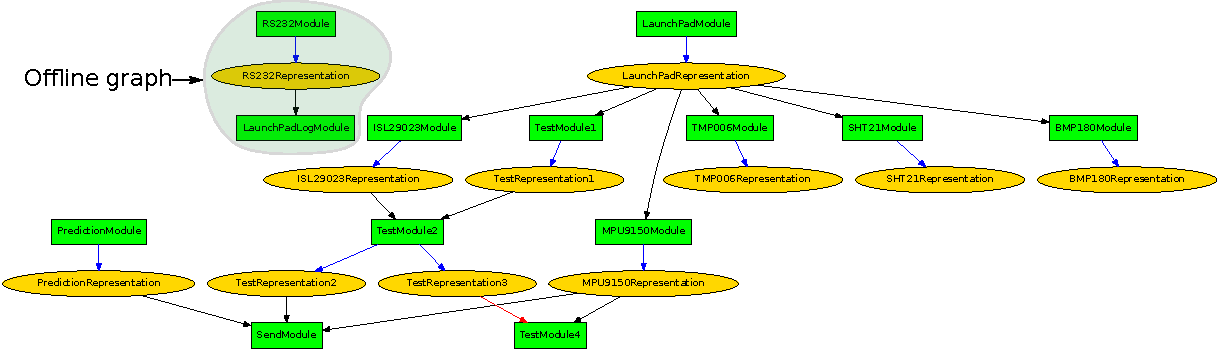
\includegraphics[width=1.0\textwidth] {framework}
 \caption{An example of modules and representations available in CSC688 Energia.}
 \label{fig:framework}
\end{figure}

The green boxes represent modules, while the yellow ellipses represent the representations. As an
example, the module {\sf MPU9150Module} contains logic to read/write from MPU-9150 Nine-Axis
(Gyro+Accelerometer+Compass) MEMS MotionTracking
device\footnote{\url{http://www.invensense.com/mems/gyro/mpu9150.html}} on the sensor hub booster
pack. The representation {\sf MPU9150Representation} contains all the values that the module
{\sf MPU9150Module} would like to share with other modules. In this graph, {\sf TestModule4}
requests
values from {\sf MPU9150Representation} to implement its logic. A module can provide multiple
representations as shown in the module {\sf TestModule2}. The blue arrows shows the provided
representations, the black arrows show the requested representations, and the red arrows show the
used representations.

There are two graphs in the figure; \begin{inparaenum}[(1)] \item the ``offline graph'' will be
executed offline, \item while the rest
of the graph, ``online graph'', will be executed on the devices\end{inparaenum}. We have shown only
two graphs in
this figure; in reality, one can keep up to $N$ number of graphs. The end uses of the software only
requires to write modules and representations, while the framework will compute the
topologically sorted graph out of the nodes. This will be computed once online/offline, and the
nodes in the queue will be executed one after the other. If there were to be cycles in the graph,
the framework will detect them and indicate them to the users.

The module {\sf PredictionModule} uses {\sf
RLLib}\footnote{\url{https://github.com/samindaa/RLLib}} library to learn, predict, and control
online on supervised and reinforcement learning problems. It provides
the representation {\sf PredictionRepresentation}. There exists a module {\sf SendModule} to send
values of the representations to offline modules. This is useful during the development phases of
a project. The module {\sf RS232Module} reads the data values that is send from {\sf SendModule}.
Please refere  to appendix for more information on implementations and
examples of the framework.

\section{Approach}
TODO:

\section{Experiments \& Results}
TODO:

\section{Related Work}
TODO:

\section{Conclusion}
TODO:

\bibliographystyle{splncs03}
\bibliography{references}

\section*{Appendix: Implementation}
\label{appendix:Implementation}
CSC688 Energia framework primarily consists of three files: \begin{inparaenum}[(1)] \item
\label{fmw:A} {\sf Template.h}; \item \label{fmw:B} {\sf Framework.h}; and \item \label{fmw:C} {\sf
Framework.cpp}\end{inparaenum}. A practitioner can only need to use these three files to get the
complete functionality of the framework. The framework has been tested on Taxas Instruments MSP430,
Stellaris, and the Tiva C LaunchPad boards. In order to compile the project:

\begin{itemize}
 \item Online (microcontrollers):
\begin{enumerate}
\item connect the microcontroller,
\item download the latest Energia distribution that matches to the host machine,
\item open {\sf csc688.ino} file, and 
\item compile and upload the {\sf csc688.elf} file to the microcontroller.
\end{enumerate}

\item Offline:
\begin{enumerate}
\item start {\sf ./configure\_offline} script to generate make file,
\item execute command {\sf make},
\item change the directory to {\sf build}, and 
\item execute the binary {./offline\_csc688}.
\end{enumerate}

\item Visualizations:
\begin{enumerate}
\item our visualization uses QT4 library. Therefore, download the latest QT4 library to your host
system,
\item change the directory to {\sf viz},
\item execute command {\sf qmake viz.pro},
\item execute command {\sf make},
\item change the directory to {\sf build}, and 
\item execute the binary {\sf viz}.
\end{enumerate}

\end{itemize}


To write modules and representations, the practitioner needs to include the three C\texttt{++}
files \ref{fmw:A}, \ref{fmw:B}, and \ref{fmw:C}. The following example shows the implementation
of the module {\sf TestModule1} and the representation {\sf TestRepresentation1} in Figure
\ref{fig:framework}.

\begin{figure}[!ht]
\begin{center}
\begin{minted}[mathescape, linenos=false, fontsize=\small]{c++}
// -----------------------------------------------------------------
#pragma once

#include "Template.h"

REPRESENTATION(TestRepresentation1)
class TestRepresentation1: public TestRepresentation1Base
{
public:
  bool rightButton, leftButton;
  TestRepresentation1() :
    rightButton(false), leftButton(false)
  {
  }
};
// ------------------------------------------------------------------
\end{minted}
\end{center}
\captionof{listing}{{\sf TestRepresentation1.h}}
\label{list:TestRepresentation1.h}
\end{figure}

Listing \ref{list:TestRepresentation1.h} shows the implementation of the representation {\sf
TestRepresentation1}. This representation shares the button state information of Tiva C among
modules. {\sf Template.h} C\texttt{++} header file provides the macro {\sf REPRESENTATION} to
register the representation with the framework, only if, a module provides the given
representation. 

\begin{figure}[!ht]
\begin{center}
\begin{minted}[mathescape, linenos=false, fontsize=\small]{c++}
// -----------------------------------------------------------------
#pragma once

#include "Template.h"
#include "LaunchPadRepresentation.h"
#include "TestRepresentation1.h"

MODULE(TestModule1)
  REQUIRES(LaunchPadRepresentation)
  PROVIDES(TestRepresentation1)
END_MODULE

class TestModule1: public TestModule1Base
{
  public:
    void update(TestRepresentation1& theTestRepresentation1);
}; 
// -----------------------------------------------------------------
\end{minted}
\end{center}
\captionof{listing}{{\sf TestModule1.h}}
\label{list:TestModule1.h}
\end{figure}

Listing \ref{list:TestModule1.h} shows the header file {\sf TestModule1.h}. This class schedules
the functionalities of a module. {\sf Template.h} defines the macros {\sf MODULE}, {\sf REQUIRES},
{\sf PROVIDES}, {\sf USES}, {\sf END\_MODULE}, and {\sf MAKE\_MODULE}.  {\sf REQUIRES} requests a
representation from another module, while {\sf PROVIDES} provides a representation from a given
module. {\sf USES} requests a representation from anywhere in the graph, without infringing the
topology of the topologically sorted graph. {\sf MODULE} and {\sf END\_MODULE} generates a base
class (e.g.,{\sf TestModule1Base}) for the module (e.g., {\sf TestModule1}) that will be used by the
framework. Since, this module provides the representation {\sf TestRepresentation1}, it needs to
implement the method \mintinline{c++}{public: void update(TestRepresentation1&
theTestRepresentation1)}. This module also requires the representation {\sf
LaunchPadRepresentation}. According to Figure \ref{fig:framework}, it is provided by the module
{\sf LaunchPadModule}. 


\begin{figure}[!ht]
\begin{center}
\begin{minted}[mathescape, linenos=false, fontsize=\small]{c++}
// -----------------------------------------------------------------
#include "TestModule1.h"

void TestModule1::update(TestRepresentation1& theTestRepresentation1)
{
  theTestRepresentation1.leftButton = theTestRepresentation1.rightButton = false;
#if defined(ENERGIA)
  if (digitalRead(PUSH1) == LOW)
    theTestRepresentation1.leftButton = true;
  if (digitalRead(PUSH2) == LOW)
    theTestRepresentation1.rightButton = true;
#endif
}

MAKE_MODULE(TestModule1)
// -----------------------------------------------------------------
\end{minted}
\end{center}
\captionof{listing}{{\sf TestModule1.cpp}}
\label{list:TestModule1.cpp}
\end{figure}


Listing \ref{list:TestModule1.cpp} shows the implementation of the module {\sf TestModule1}.  The
macro {\sf MAKE\_MODULE} registers the module {\sf TestModule1} with the framework. According to
Figure \ref{fig:framework}, the module {\sf TestModule2} requests representations provided by {\sf
TestModule1}. Please refer to the documentation of CSC688 Energia for more examples and usages
(\url{https://github.com/samindaa/csc688}).  




\end{sloppy}
\end{document}